\section{Trabalhos Relacionados}\label{sec:rel}

\subsection{Redução de Dimensionalidade Automática}

Os métodos de redução de dimensionalidade automática 

\subsection{Redução de Dimensionalidade Interativa}

% representações diretas são simples mas não escalam (Representações Diretas)
% vamos tentar fazer as diretas escalar arranjando as dimensões (Arranjo de Dimensões)
% nem arranjando dá pra ver tudo então o jeito é reduzir (Redução de Dimensionalidade)
% redução pode ser pouco intuitiva e pode tamém esconder features locais (Features Locais)
% cada um tem o seu defeito então vamos tentar juntar tudo pra ver se vai (União de Métodos)
% é legal também falar de ideias alternativas (Métodos Alternativos)

% Os métodos de \emph{Feature Selection} buscam compor um      subconjunto das dimensões originais  que contém atributos    realmente relevantes para a análise~\cite{Molina2002}. No    entanto, foi mostrado que encontrar o subconjunto ideal é um problema NP-completo~\cite{Blum1988}. Assim, esses métodos   trabalham com base em heurísticas e não garantem que o       conjunto ótimo será encontrado. A maioria desses métodos     apresenta complexidade computacional quadrática ou superior, logo não são escaláveis para   conjuntos de dados com centenas ou milhares de               dimensões~\cite{Liu2005}.

% O processo de \emph{Feature Extraction} reduz a              dimensionalidade de um conjunto de dados por meio de         combinações dos atributos originais. O resultado obtido por  esses métodos nem sempre é de fácil compreensão, pois a      combinação entre os atributos pode não apresentar relação    com o domínio dos dados~\cite{Jeong2009}. Outra limitação de alguns desses métodos é a necessidade dos dados seguirem uma distribuição normal, fato que nem sempre pode ser garantido  e exige que métodos mais complexos sejam                     utilizados~\cite{Fodor2002}.A

% It has already been observed that only the least complex (eg. O(n)) schemes are able to cope with ‘large’ data sets as proposed. For this reason, the sim- pler schemes here are described more thoroughly here than might have been expected.

A literatura em redução de dimensionalidade é extensa e os métodos desenvolvidos apresentam grande diversidade em relação a aspectos matemáticos e computacionais. Buscando uma melhor contextualização, esta seção aborda apenas trabalhos que buscam de alguma forma utilizar representações visuais para a execução desta tarefa.

\subsection{Representações Tradicionais}

% Scatter plots e PC %%%%

A técnica visual mais simples para a investigação de atributos de uma base de dados é a matriz de gráficos de dispersão~\cite{Becker1987}, mais conhecidos como \textit{scatter plots}. Um \textit{scatter plot} permite a investigação da correlação entre duas variáveis ao plotar os pontos de dados em dois eixos ortogonais. Como mostra a Figura~\ref{fig:smatrix}, uma matriz de \textit{scatter plots} simplesmente organiza as combinações possíveis entre as variáveis em uma estrutura ordenada. 

\begin{figure}[h!]
  \centering
  \begin{subfigure}[b]{0.5\textwidth}
    \centering
    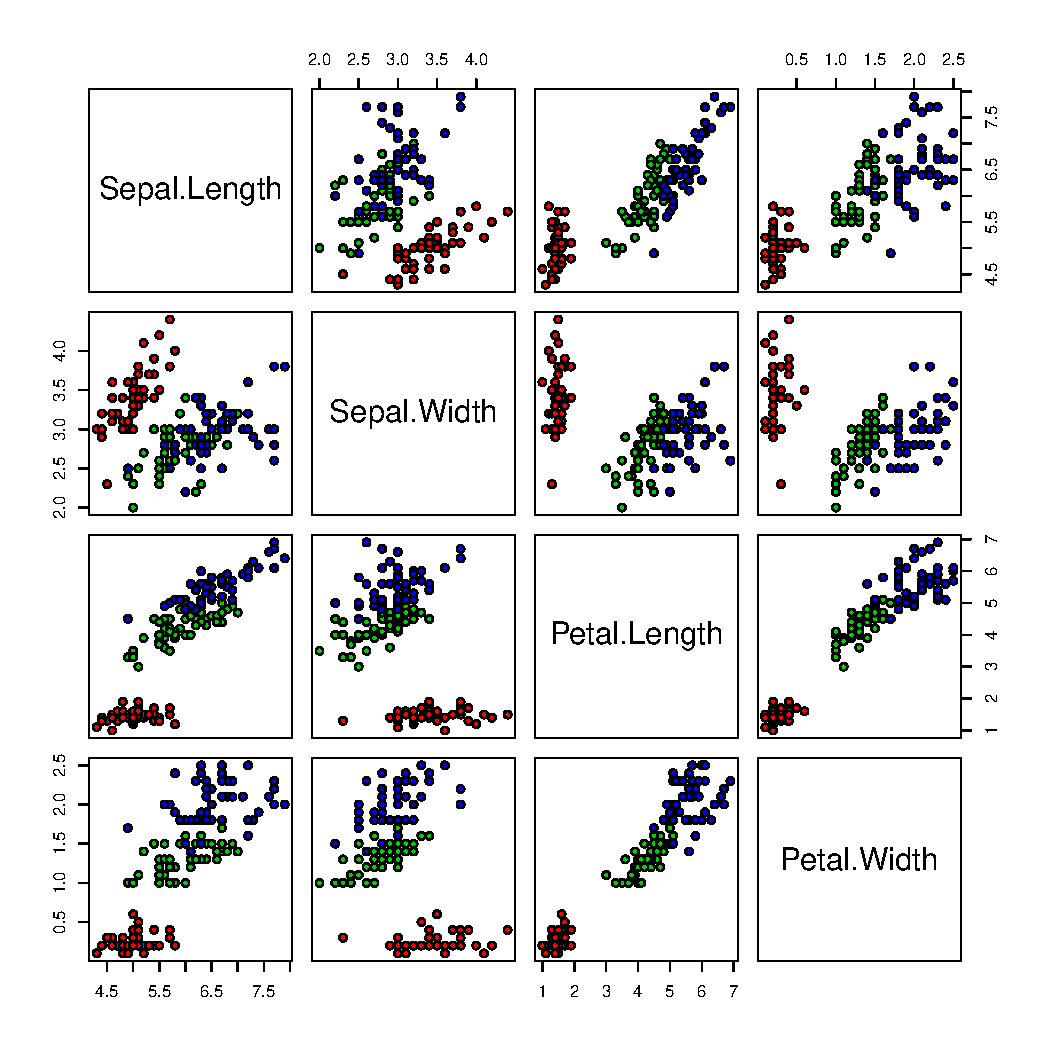
\includegraphics[width=\textwidth]{images/smatrix.pdf}
    \caption{}
    \label{fig:smatrix}
  \end{subfigure}%
  ~ %add desired spacing between images, e. g. ~, \quad, \qquad etc.
  \begin{subfigure}[b]{0.5\textwidth}
    \centering
    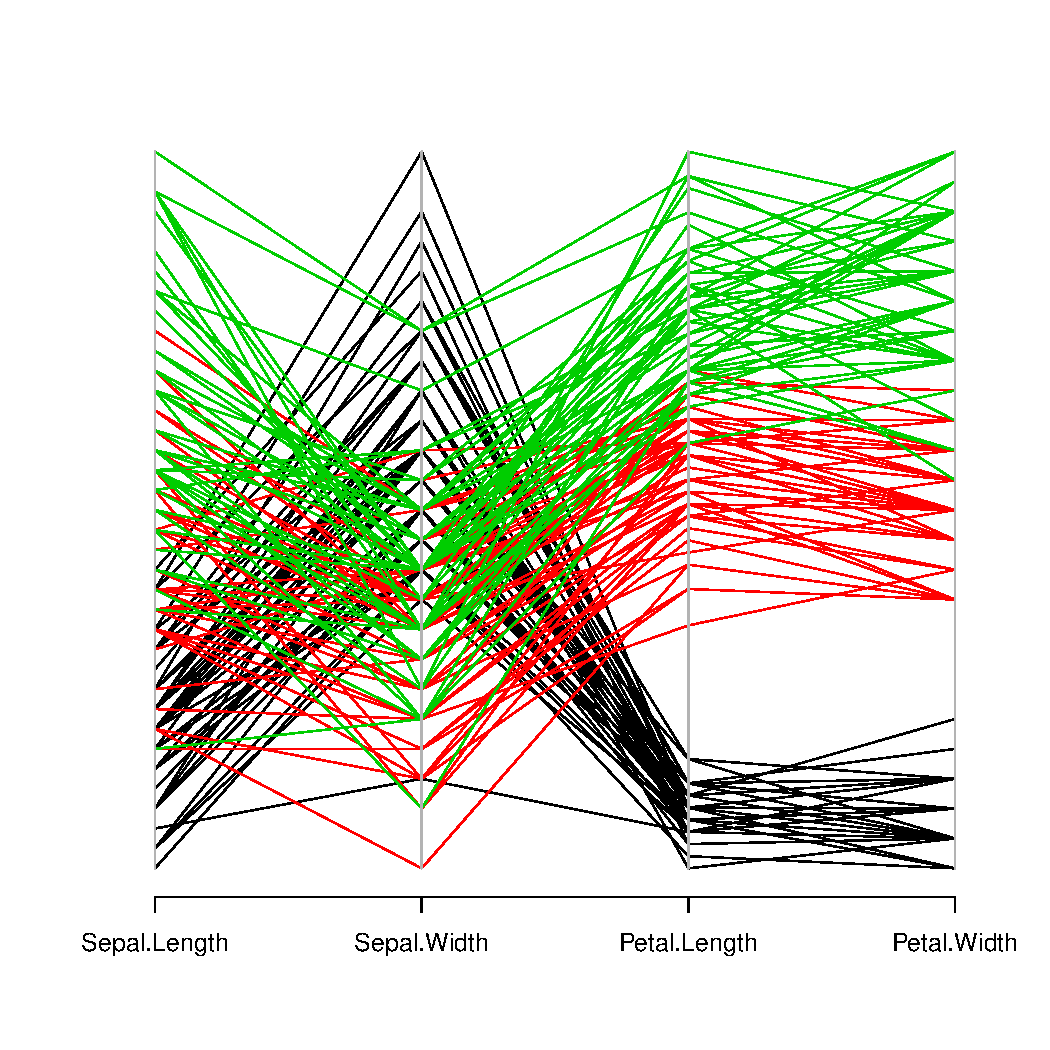
\includegraphics[width=\textwidth]{images/parcoord.pdf}
    \caption{}
    \label{fig:parcoord}
  \end{subfigure}
  \caption[Exemplos de matriz de scatter plot e coordenadas paralelas.]{(a) Exemplo de matriz de scatter plot, correlação posicitava entre basd ad}
\end{figure}

No entanto, nota-se dois problemas principais em relação à esta técnica. Primeiramente, a representação visual não é capaz de lidar com um grande número de dimensões, pois a matriz pode exigir demasiado espaço para representar adequadamente cada gráfico. Outro problema está relacionado ao fato de que não é possível observar correlações além do que bivariadas, devido ao fato das análises serem realizadas para pares de atributos individualmente. 

Outra técnica muito utilizada para este tipo de análise é a chamada coordenadas paralelas~\cite{PC1990}. Nesta técnica as dimensões são representadas por um conjunto de retas paralelas e os itens por linhas que cortam essas retas. Observando a Figura~\ref{fig:parcoord} nota-se que uma única representação visual contém todas as dimensões. Porém, a ordem das retas paralelas afeta diretamente no resultado da técnica.


Porém, essas técnicas sofrem do problema de baixa escalabilidade tanto para o número de itens quanto para o número de atributos da base de dados. Alguns trabalhos buscaram tratar este problema em relação ao número de itens \cite{Heinrich2009,Kandogan00} (citar um de scatter contínuo). No entanto, ainda existe uma grande dificuldade em lidar com conjuntos de dados que possuem um grande número de dimensões. Star coordinates consegue mostrar mais dimensões, porém é suscetível à ambiguidades, pois dois pontos com atributos diferentes podem ser posicionados na mesma posição por mera coincidência.

% Quando o número de dimensões extrapola as dezenas não é trivial ordenar adequadamente os atributos, logo a tarefa de encontrar relações entre os atributos torna-se inviável. 

% O problema das duas é praticamente o mesmo. Enxugar o texto falando geral pra ambos.

% Pixel Oriented

\subsection{Redução de dimensionalidade} 

As presented in this section, a large number of dimensionality reduc- tion techniques and systems exist. For several, the relationship be- tween the original and reduced data set is not intuitive and the user has little or no control over the reduction. Moreover, many techniques are limited either to focusing on pairs of variables or to only taking a sin- gle quality metric into consideration. 

A common approach to visualization of data sets with large numbers of variables is to precede the visualization with some dimensionality reduction, visually representing the data set in a lower dimensional space preserving some of the structures of the original data set.

Some of the more popular dimensionality reduction methods are
Principal Components Analysis (PCA) [11], which preserves variance by extracting a number of principal components, Multidimensional Scaling (MDS) [15], preserving dissimilarities, and Self Organizing Maps (SOM) [13], preserving topological and metric relationships. 


% PCA

Dentre os métodos que combinam métodos estatísticos e visuais para a exploração de atributos de uma base de dados, PCA (\textit{Principal Component Analysis)}~\cite{Wold1987} é o mais tradicional. Interpretando os autovalores e autovetores resultantes deste método é possível investigar as relações entre dimensões. 

Esta distorção da dimensionalidade confunde os usuários, pois as propriedades das novas dimensões não são necessariamente análogas ao problema real.

% iPCA

provides an interactive in- terface where the user can manipulate the weights of data attributes in order to figure out which attributes con- tribute most to the principal component directions

% PCVG

An example of variable grouping is the Principal Component Variable Grouping (PCVG) presented in [10]. PCVG is based on PCA but uses the principal components to group the original variables.

% Biplots

% MDS 

A large class of dimensionality reduction techniques have the
holistic goal of determining a new set of synthetic dimensions that express most or all of the structure in the input dataset using fewer total dimensions than the original representation. For example, Principal Components Analysis (PCA) constructs synthetic dimensions that are a linear combination of some subset of the original ones [9], and other methods such as multidimensional scaling (MDS) use nonlinear combinations [1]. The goal of these tech- niques is to reveal hidden variables, for example where the phenomenon of interest could only be measured indirectly. In these cases, the data reside in a lower dimensional manifold whose coordinate axes are best represented as a linear or nonlinear combination of the input dimensions.

Porém seu resultado é de difícil compreensão (13-Dust). 

% Steerable MDS 

In [24] an interactive system is presented where the user can guide the MDS process during computation and select local regions of interest to focus the computational effort on.
the relationship between the original and reduced sets of variables is usu- ally not intuitive

% SOM

\subsection{União entre Métodos}

Métodos mais sofisticados têm sido desenvolvidos para lidar com as novas exigências impostas pelos grandes conjuntos de dados. Estes métodos combinam diversas técnicas em um sistema integrado e possibilitam a interação do usuário para viabilizar a exploração de conjuntos de dados que possuem um elevado número de atributos.

% VAR %%%%

A técnica VaR (Value and Relation)~\cite{Patro}, por exemplo, une os conceitos de projeção multidimensional e glifos para representar as dependências das dimensões de uma base de dados. Como mostra a Figura~\ref{fig:var1}, cada glifo representa uma dimensão e de acordo com seus posicionamentos no plano, o usuário pode compreender quais dimensões se relacionam entre si e assim, pode escolher somente atributos de real interesse e não redundantes para análises mais detalhadas.

\begin{figure}[h!]
  \centering
  \begin{subfigure}[b]{0.5\textwidth}
    \centering
    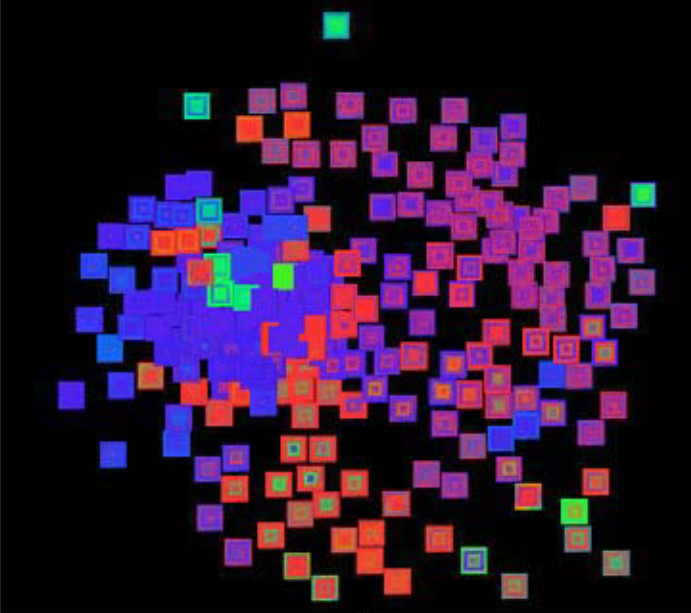
\includegraphics[width=\textwidth]{images/var1.png}
    \caption{}
    \label{fig:var1}
  \end{subfigure}%
  ~ %add desired spacing between images, e. g. ~, \quad, \qquad etc.
  \begin{subfigure}[b]{0.475\textwidth}
    \centering
    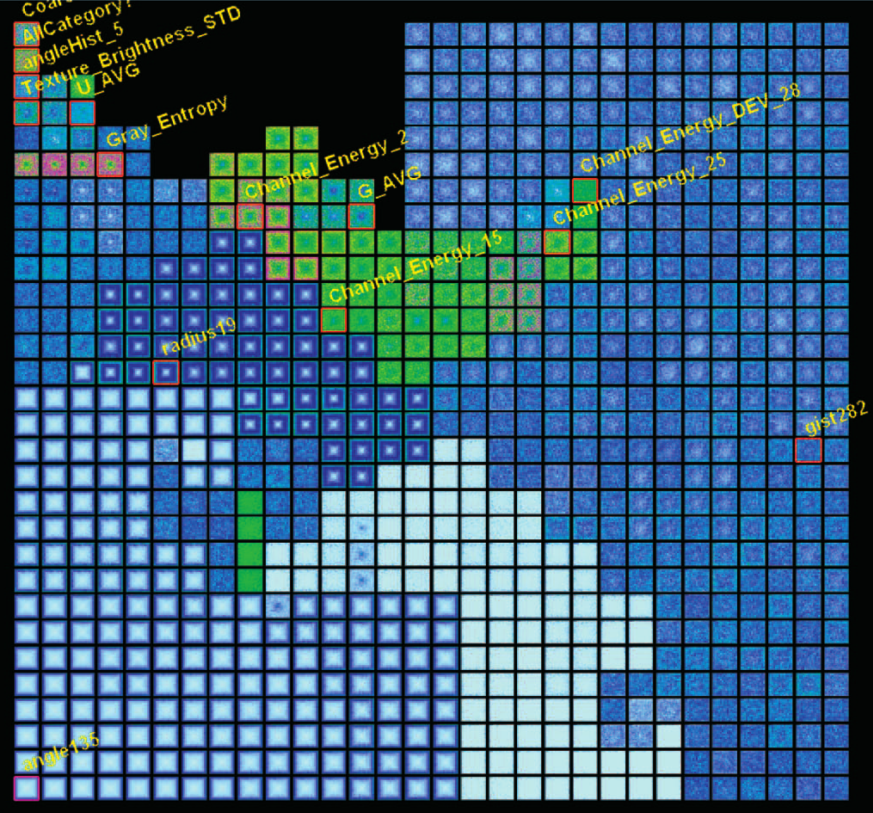
\includegraphics[width=\textwidth]{images/var2.png}
    \caption{}
    \label{fig:var2}
  \end{subfigure}
  \caption[VaR: Value and Relation]{(a) Exemplo da técnica VaR para um conjunto de $50.000$ itens e $361$ dimensões. Cada dimensão é representada por um glifo e seus posicionamentos refletem a similaridade entre as dimensões, de modo que glifos que se encontram próximos indicam atributos que apresentam alguma relação entre si. É possível notar certas sobreposições entre os glifos, condição que pode dificultar as análises realizadas pelo usuário. (b) Exemplo de representação alternativa proposta como extensão da técnica VaR para um conjunto de 11.413 itens e 838 dimensões. O principal objetivo da representação é evitar a sobreposições de glifos ocorrente na versão anterior da técnica.}
\end{figure}

Observando a Figura~\ref{fig:var1} é possível notar que o uso de glifos faz com que ocorram sobreposições, pois cada glifo requer um espaço relativamente grande para que seja observado adequadamente. A sobreposição dificulta as análises de regiões de interesse e pode fazer com que o usuário alcance conclusões inválidas, devido a oclusão de algum elemento fundamental. Buscando tratar este problema~\citeauthor{Yang2007} desenvolveram a extensão~\cite{Yang2007} ilustrada na Figura~\ref{fig:var2} para a técnica VaR, onde apresentaram alternativas para a projeção de glifos no plano. No entanto, diferentemente das projeções, as alternativas propostas não são capazes de transmitir a magnitude da similaridade entre as dimensões.


% Calculo de similaridade, inventou uma técnica e a comparou com euclidiana. Não mencionou ter testado com outras, por exemplo, as bem definidas de ML.

% Dar exemplos da sobreposição e da comparação entre elementos.

% RBF %%%%

\citeauthor{Shneiderman2004} desenvolveram o framework Rank-by-Feature~\cite{Shneiderman2004} com o intuito de auxiliar a descoberta de correlações entre atributos. Eles classificam os atributos com base em critérios estatísticos definidos pelo usuário e possibilitam a construção de projeções uni ou bidimensionais para a avaliação da classificação realizada. Certas análises podem exigir demasiado esforço do usuário, devido à necessidade de se explorar individualmente cada dimensão ou avaliar par a par as relações entre atributos. Com a ocorrência de dependências não lineares este problema torna-se ainda maior e o usuário pode facilmente se perder em suas análises e não extrair novos conhecimentos dos resultados.

% Brushing %%%%

A exploração das relações entre as dimensões não precisa estar vinculada somente a representações visuais dos atributos do conjunto de dados. \citeauthor{Turkay2011}~\cite{Turkay2011} propuseram um método de múltiplas visões que permite que o usuário interaja tanto com as dimensões quanto com os itens da base de dados. O principal mecanismo de interação é a seleção que se reflete em outras visões e permite que se visualize, por exemplo, as dimensões que melhor representam subconjuntos dos dados. Uma das limitações deste trabalho é falta de medidas que consideram pares de dimensões, como medidas de correlação, o que dificulta a observação de dependências entre os atributos.   

% VHDR %%%%

Em busca de construir espaços de baixa dimensionalidade mais intuitivamente do que pelo uso de métodos automáticos, \citeauthor{Yang2003} desenvolveram um método de redução de dimensionalidade chamado VHDR (Visual Hierarchical Dimensions Reduction)~\cite{Yang2007}. Este método utiliza a similaridade entre pares de dimensões para construir uma organização hierárquica dos atributos. O processo é ortogonal ao agrupamento de itens, assim é possível identificar grupos de dimensões com características semelhantes. Porém, para conjuntos de dados com mais do que algumas dezenas de dimensões, as representações visuais utilizadas podem se tornar poluídas. Os autores mencionam que algoritmos adaptados da área de agrupamentos de dados poderiam ser utilizados para gerar a hierarquia de dimensões, no entanto eles adotaram uma abordagem mais simples para medir a similaridade entre dimensões: medem a diferença entre os valores normalizados dos atributos e verificam se esta diferença é menor do que um \textit{threshold} pré estabelecido. Este método para o cálculo da similaridade é a grande limitação do trabalho, pois não captura dependências entre os atributos. Além disso, não são apresentadas mecanismos interativos como alternativa para o método automático de identificação de dimensões representativas de um grupo. 

% Utilizar uma figura para ilustrar o processo 

% DOSFA %%%%

The Dimension Ordering Spacing and Filtering Approach (DOSFA) [26] has evolved from VHDR and provides di- mensionality reduction based on a combination of similarity and of a given importance measure, such as variance. DOSFA is also aiming at finding a visual layout that facilitate the detection of structures within the data.

% Coord %%%%

Falo de corrgram e falo de coord, mas que o problema delas é a escabilidade

baklh aborda o problema de que subconjuntos dos dados podem apresentar características diferentes, assim em alguns casos é impossível encontrar um único conjunto de atributos que represente todos os subconjuntos adequadamente. 

% Dimstiller  %%%%

Este paper apresenta uma ferramenta que permite ao usuário definir uma sequência de ações para a exploração de grandes conjuntos de dados. Parte da combinação de diversas técnicas para permite a interação, mas não apresenta nada de novo.

% Dust and Magnet %%%%

Este paper busca fornecer a população em geral uma técnica de fácil entendimento que se baseia na metáfora de um imã.

% High-D %%%%

Utiliza conceitos de ordenação de dimensões semelhantes à Coord. MST sobre o grafo e permite que se avalie a correlação entre dimensões utilizando uma matriz.

% MP %%%%

As técnicas VHDR e DOSFA constroem uma hierarquia com base na similaridade entre as dimensões para apresentar explicitamente os relacionamentos entre os atributos e permitem que os usuários interativamente selecionem as dimensões de interesse.

Diversos trabalhos se baseiam na interação com representações visuais para investigar o processo de seleção automática e permitir que o usuário participe deste processo. 

% Smart stripes %%%%

% Guiding %%%%

Este paper propõe uma técnica para avaliação e orientação do processo de feature selection com base em métodos interativos visuais. Trata o problema de que diferentes partições das entidades dos dados podem apresentar  importâncias distintas de features. Permite que o usuário participe do processo de seleção e a investigue as dependências e interdependências entre conjuntos de features e itens.

% Melhor falar primeiro de Smart e depois falar o que Guiding fez de diferente.

\cite{May2011} parte da ideia introduzida por 14 para blabh blah. Trata os problemas gerados pela agregação estatística, ou seja, features de interesse podem ser mascaradas por outras menos interessantes. Um problema desta técnica é a necessidade de se estabelecer uma feature de referência, pois a representação visual apresenta apenas as relações de 1-n.

\clearpage
